\chapter{LibGen -{} Library Generator -{} Part 1}

\section{Introduction}
\label{ch31-intro}%\hyperlabel{ch31-intro}%

In the last chapter, I looked at the creation and use of libraries
    with Gwasl\program{Gwasl}. George and I had a bit of an
    email conversation we had about how to work around the problem of only
    exposing the required routines in the libraries we create without exposing
    the internal working routines. For example, in my small example library, I
    would only expose the various CLEAR\_xxx routines, but
    not the internal JUST\_DO\_IT routine. Also, it is not
    required to expose any of the equates used internally by the library -{}
    simply because they may conflict with your own equates used elsewhere in
    the program and because, by the time the library is assembled, the equates
    have been converted into absolute values anyway.

George mentioned editing the library source code, setting a new
    equate with a given prefix, to the routines you wish to expose, similar to
    the following:

\begin{lstlisting}[firstnumber=1,]
LB_CLEAR_SCREEN equ clear_screen
\end{lstlisting}

In the above, you can see that I've set
 LB\_CLEAR\_SCREEN equal to
 CLEAR\_SCREEN. When the symbol file is converted to
    text, it will have the following in it:

\begin{lstlisting}[firstnumber=1,]
...
CLEAR_SCREEN    EQU     *+$00000000
LB_CLEAR_SCREEN EQU     *+$00000000
JUST_DO_IT      EQU     *+$00000012
...
\end{lstlisting}

You can see, that CLEAR\_SCREEN and
 LB\_CLEAR\_SCREEN are the same. George proposed that a
    SuperBasic program could be quickly written to extract only those equates
    prefixed by, for example, `LB\_' and this extracted file could then be used
    to expose only the chosen routines.

I liked this idea, but I'm sort of wary about having to edit my
    source code and add extra equates whenever I write a new routine. Equally,
    this is an assembler tutorial and at present I'm writing about the Pointer
    Environment, so how about a useful -{} yes, the first one -{} utility to read
    in a sym\_lst file, display all the code offset equates (and only those)
    and when the user has selected the desired items, write out a valid file
    that can be included. This issue's article is that very utility!

\section{The SYM\_LST File Format}
\label{ch31-sym-lst-format}%\hyperlabel{ch31-sym-lst-format}%

Once symbol file has been converted to text by running George's
 SYM\_BIN utility, the format is quite
    simple.\footnote{It is indeed simple, but don't base any assumptions on the fact that all of George's symbol file listings will be in this format. Those produced by the Gwasl assembler's sym\_bin utility are slightly different from those created by the Gwass assembler's sym\_bin utility. Ask me how I know! Oh yes, the internal binary format of the two assemblers' sym files are different too. Shame.}
\begin{itemize}[itemsep=0pt]

\item{}Columns 0 to 29 hold the label.

\item{}Columns 30 to 35 hold ``EQU''.

\item{}Columns 36 onwards hold the equate value, or the code
        offset.

\end{itemize}

However, it matters not for this utility anyway, because all I'm
    doing is extracting the entire line from the file and adding it to a menu
    so that the user can select or deselect it at will. What does matter,
    however, is the difference between a code offset and a value in the file.
    Look again at the example above and note that my original equates simply
    show a hexadecimal value, while the code offsets show a similar hex value,
    prefixed by the two characters `*+' (Asterisk and plus). My utility,
 LibGen\program{LibGen}, only extracts the latter.

\section{LibGen}
\label{ch31-Lib-Gen}%\hyperlabel{ch31-Lib-Gen}%

I've chosen LibGen\program{LibGen} as my utility name.
    The finished screen will hopefully look very similar to the screen shot in Figure~\ref{fig:WhatLibGenShouldLookLike}

\begin{figure}[h]
\center
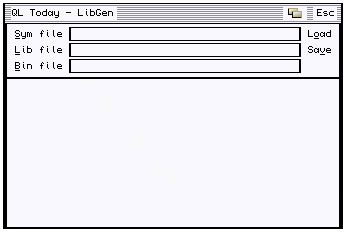
\includegraphics[width=0.65\textwidth]{Content/images/libgen_1.png}
\caption{What LibGen Should Look Like!}
\label{fig:WhatLibGenShouldLookLike}
\end{figure}


Along the top is a green/white (paper 92) caption bar which is
    simply an information window. The actual title is itself embedded in
    another small information window with white paper. The move loose item and
    the Esc loose items are embedded within the main caption bar. To keep code
    sizes to a minimum, there is no Size or Sleep loose items in this
    utility.

Moving down the screen there is a large information window with a
    black border and white paper containing the 5 loose items -{} Sym file, Lib
    file, Bin file, Load and Save, and three further information Windows, each
    with white paper and a black border.

The largest part of the window is taken up by an application window
    at the bottom. This too has white paper and a black border. This is where
    we will hold the code offset lines from the symbol file.

In operation, you click on `sym file' to allow the name of the
    sym\_lst file in question to be loaded. If the file loads, the `\_sym\_lst'
    extension is removed and replaced with `\_lib' for the `Lib file' and
    `\_bin' for the `Bin file'. You can, however, edit these auto-{}generated
    names by hitting the appropriate loose item.

When happy with the names, hit the `Load' loose item to read in the
    file. The application window will fill up with appropriate options from
    the file and you will be able to choose the ones you wish to keep. By
    default everything is selected, you only need to deselect the ones you
    don't want to keep. I'm working on the assumption that you will want to
    keep more than you don't, so it should be easier to deselect the few than
    select the many.

Once happy with your selection, hit the `Save' loose item and the
    selected entries will be copied to the `Lib file' along with a line to
    include the `Bin file', as follows:

\begin{lstlisting}[firstnumber=1,]
CLEAR_SCREEN  EQU     *+$00000000
CLEAR_TOP     EQU     *+$00000004
CLEAR_BOTTOM  EQU     *+$00000008
CLEAR_TO_EOL  EQU     *+$0000000C
CLEAR_LINE    EQU     *+$00000010

              lib     win1_gwasl_libs_lib_cls_bin
\end{lstlisting}

Now all you need to do is add one line to your program, as
    follows:

\begin{lstlisting}[firstnumber=1,]
              in    win1_gwasl_libs_lib_cls_lib
\end{lstlisting}

Hopefully, this is a lot easier than editing source code, adding
    extra equates, and running a SuperBasic program to extract them and so
    on.

\section{Window Design}
\label{ch31-lib-gen-window-design}%\hyperlabel{ch31-lib-gen-window-design}%

Make sure that you download the latest versions of
 SETW\program{SETW} and Easy PEasy\program{EasyPEasy}     from \url{http://gwiltprogs.info/page2.htm} as George has recently updated these to make our lives much easier. We
    will be using the new features of Easy PEasy\program{EasyPEasy} in
    this utility. We begin by designing our window with
 SETW\program{SETW}. Now, contrary to my own instructions
    above, I have to declare here that I'm not yet using the latest version of
 SETW\program{SETW}! I'm also abbreviating the prompts etc in
    the following steps to try and keep coding to a minimum.
\begin{enumerate}
\item{Enter a name, I used libgenwin for mine, but feel free to make
        up your own.
}
\item{Enter the following text objects by pressing the `N' key, then
        typing in the text:
\begin{itemize}[itemsep=0pt]

\item{}QL Today -{} LibGen


\item{}Esc


\item{}Sym file


\item{}Lib file


\item{}Bin file


\item{}Load


\item{}Save

\end{itemize}

Press ESC when done.
}
\item{For the sprites, blobs and patters, simple press Esc as we have
        none of those.
}
\item{There is one single main window.
}
\item{There are 7 loose items within it.
}
\item{There are 6 information windows.
}
\item{Information windows 1 to 4 have no objects, number 5 has one,
        and number 6 has none.
}
\item{There will be one application window, but it has no menu items.
        (We will build the menu dynamically.)
}
\item{The main window has the following attributes:
\begin{itemize}[itemsep=0pt]

\item{}Shadow size 2


\item{}Border size 1, border colour is QL Black.


\item{}Paper colour is QL White.


\item{}Select the default arrow sprite for the pointer.

\end{itemize}
}
\item{When prompted, twice, to select default settings for loose
        items, chose `N' both times. We will enter our own settings.
}
\item{The current item border size is 1 and the colour is QL
        Black.
}
\item{Unavailable attributes are:
\begin{itemize}[itemsep=0pt]

\item{}Background colour is QL White.


\item{}Ink colour is QL Grey.

\end{itemize}
}
\item{Available attributes are:
\begin{itemize}[itemsep=0pt]

\item{}Background colour is QL White.


\item{}Ink colour is QL Black.

\end{itemize}
}
\item{Selected attributes are:
\begin{itemize}[itemsep=0pt]

\item{}Background colour is QL Green.


\item{}Ink colour is QL Black.

\end{itemize}
}
\item{For the 7 loose items, set them up as follows:
\begin{enumerate}[itemsep=0pt]

\item{}Type is text, choose the `Esc' text, no selection
            key.


\item{}Type is text, choose the `Esc' text again, no selection key.
            We will fix this later as we need a sprite.


\item{}Type is text, choose the `Sym file' text, selection key is
            `S' and underlined.


\item{}Type is text, choose the `Lib file' text, selection key is
            `L' and underlined.


\item{}Type is text, choose the `Load' text, selection key is `O'
            and underlined.


\item{}Type is text, choose the `Save' text, selection key is `V'
            and underlined.


\item{}Type is text, choose the `Bin file' text, selection key is
            `B' and underlined.

\end{enumerate}

Loose item 2 uses the same `Esc' text as loose item 1 but we
        will fix this in the code that gets generated. I haven't yet found a
        way of getting the standard sprites into a
 SETW generated program.
}
\item{For the 6 information windows, set them up as follows:
\begin{enumerate}[itemsep=0pt]

\item{}Border size zero, paper QL 92.


\item{}Border size 1, colour QL Black, paper QL White.


\item{}Border size 1, colour QL Black, paper QL White.


\item{}Border size 1, colour QL Black, paper QL White.


\item{}Border size 0, paper QL White. When prompted for an object,
            choose Text `QL Today -{} LibGen', set the ink to QL Black and the
            two CSizes to zero.


\item{}Border size 1, colour QL Black, paper QL White.

\end{enumerate}
}
\item{The application window needs the following:
\begin{itemize}[itemsep=0pt]

\item{}Border size 1.


\item{}Colour QL Black.


\item{}Paper QL White.


\item{}Choose the standard arrow sprite.


\item{}Set the selection key to TAB.

\end{itemize}
}
\item{There now follows a session of pressing arrow keys and F2 etc to
        size and position all the loose items, information windows to build
        our window. The main window itself is first:
\begin{itemize}[itemsep=0pt]

\item{}The size is 336 by 224.


\item{}The window is not a variable one.


\item{}The pointer origin is 50 by 37.

\end{itemize}
}
\item{The 7 loose items should be sized and positioned as
        follows:
\begin{enumerate}[itemsep=0pt]

\item{}24 by 13 at 308 by 3.


\item{}24 by 13 at 278 by 3.


\item{}50 by 14 at 8 by 23.


\item{}50 by 14 at 8 by 39.


\item{}28 by 14 at 300 by 23.


\item{}28 by 14 at 300 by 39.


\item{}50 by 14 at 8 by 55.

\end{enumerate}
}
\item{The 6 information windows should be sized and positioned as
        follows:
\begin{enumerate}[itemsep=0pt]

\item{}336 by 20 at 0 by 0.


\item{}332 by 53 at 2 by 20.


\item{}228 by 12 at 66 by 24.


\item{}228 by 12 at 66 by 40.


\item{}106 by 13 at 6 by 3. When prompted for the object, position
            it at 0 by 1.


\item{}228 by 12 at 66 by 56.

\end{enumerate}
}
\item{The application window should be 332 by 148 and positioned at 2
        by 75.
}
\end{enumerate}

You will notice that the screen looks a bit cluttered and the
    program prompts can be hard to see under all the loose items, information
    windows etc. When you are finished, the window will be displayed on
    screen. If it looks ok, all well and good, if not, don't worry, it can be
    fixed in the generated code, which should look as follows. We need to do
    some editing as well, but I'll cover that below.

\begin{lstlisting}[firstnumber=1,caption={LibGenWin\_asm}]
SYS_SPR dc.w    0,1,2,3,4,5,6,7,8,9,10,11,12,13
        dc.w    14,15,16,17,18,19,20,21,22,23,24
        dc.w    25,26,27,28,29,30,31,32,33,34,35
        dc.w    36,37

txt0    dc.w    txt0_e-2-txt0
        dc.b    "QL Today - LibGen"
txt0_e  ds.b    0
        ds.w    0

txt1    dc.w    txt1_e-2-txt1
        dc.b    "Esc"
txt1_e  ds.b    0
        ds.w    0

txt2    dc.w    txt2_e-2-txt2
        dc.b    "Sym file"
txt2_e  ds.b    0
        ds.w    0

txt3    dc.w    txt3_e-2-txt3
        dc.b    "Lib file"
txt3_e  ds.b    0
        ds.w    0

txt4    dc.w    txt4_e-2-txt4
        dc.b    "Bin file"
txt4_e  ds.b    0
        ds.w    0

txt5    dc.w    txt5_e-2-txt5
        dc.b    "Load"
txt5_e  ds.b    0
        ds.w    0

txt6    dc.w    txt6_e-2-txt6
        dc.b    "Save"
txt6_e  ds.b    0
        ds.w    0

app_list0
        dc.w    appw0-*
        dc.w    0

appw0
        dc.w    332       xsize
        dc.w    148       ysize
        dc.w    2         xorg
        dc.w    75        yorg
        dc.w    0         flag
        dc.w    1         borw
        dc.w    0         borc
        dc.w    7         papr
        dc.w    0         pspr *
        dc.w    0         setr *
        dc.w    0         draw *
        dc.w    ahit0-*   hit *
        dc.w    0         cntrl *
        dc.w    0         nxsc
        dc.w    0         nysc
        dc.b    9         skey
        dc.b    0         spr1

pobl4
        dc.w    102       xsize
        dc.w    10        ysize
        dc.w    0         xorg
        dc.w    1         yorg
        dc.b    0         type
        dc.b    0         spar
        dc.l    0         spce
        dc.w    txt0-*    pobj *
        dc.w    -1

infw0
        dc.w    336       xsize
        dc.w    20        ysize
        dc.w    0         xorg
        dc.w    0         yorg
        dc.w    0         flag
        dc.w    0         borw
        dc.w    0         borc
        dc.w    92        papr
        dc.w    0         pobl *

        dc.w    332       xsize
        dc.w    53        ysize
        dc.w    2         xorg
        dc.w    20        yorg
        dc.w    0         flag
        dc.w    1         borw
        dc.w    0         borc
        dc.w    7         papr
        dc.w    0         pobl *

        dc.w    228       xsize
        dc.w    12        ysize
        dc.w    66        xorg
        dc.w    24        yorg
        dc.w    0         flag
        dc.w    1         borw
        dc.w    0         borc
        dc.w    7         papr
        dc.w    0         pobl *

        dc.w    228       xsize
        dc.w    12        ysize
        dc.w    66        xorg
        dc.w    40        yorg
        dc.w    0         flag
        dc.w    1         borw
        dc.w    0         borc
        dc.w    7         papr
        dc.w    0         pobl *

        dc.w    106       xsize
        dc.w    13        ysize
        dc.w    6         xorg
        dc.w    3         yorg
        dc.w    0         flag
        dc.w    0         borw
        dc.w    0         borc
        dc.w    7         papr
        dc.w    pobl4-*   pobl *

        dc.w    228       xsize
        dc.w    12        ysize
        dc.w    66        xorg
        dc.w    56        yorg
        dc.w    0         flag
        dc.w    1         borw
        dc.w    0         borc
        dc.w    7         papr
        dc.w    0         pobl *

        dc.w    -1        end

\end{lstlisting}

So far, so good. Nothing in the above should differ from what you
    typed into SETW\program{SETW}. If anything has been created
    in error, you can adjust it in the above. Coming next is the loose items
    definitions and it is here that we have to change a few things.

In the first loose item below, the Selection Key has been set to 3.
    When we created this loose item in SETW\program{SETW}, we
    didn't select a selection key for it. The first loose item is for Esc, and
    we give it a selection key of 3, which corresponds to the Cancel event
    code.

The second of the loose items was created originally pointing at the
    same `Esc' text as the first, however, we need to use a system sprite to
    indicate that this is the Move loose item, and also, because we are using
    a sprite and not a text object, we need to change the object type. And
    finally, the selection key is set to the event code of 5 for Move. (All
    changes below have comments.)

Note that when using a system sprite, the sprite pointer has to
    point, relatively, at a word containing the sprite number.

\begin{lstlisting}[firstnumber=last,caption={LibGenWin\_asm - Loose Items}]
litm0
        dc.w    24,13     xsize, ysize
        dc.w    308,3     xorg, yorg
        dc.b    0,0       xjst, yjst
        dc.b    0,3       type, skey   ; SKEY = ESC event.
        dc.w    txt1-*    pobj *
        dc.w    0         item
        dc.w    afun0_0-* pact *

        dc.w    24,13     xsize, ysize
        dc.w    278,3     xorg, yorg
        dc.b    0,0       xjst, yjst
        dc.b    2,5       type, skey   ; SKEY = MOVE, TYPE = sprite
        dc.w    sys_spr+12-*  pobj *   ; POBJ = move sprite.
        dc.w    1         item
        dc.w    afun0_1-* pact *        
\end{lstlisting}

The next two loose items have their horizontal justification set to
    -{}1 which means `justify right'. Again, the changes from the code generated
	    by SETW\program{SETW} is highlighted in the comments.

\begin{lstlisting}[firstnumber=last,caption={LibGenWin\_asm - Loose Items - Continued}]
        dc.w    50,14     xsize, ysize
        dc.w    8,23      xorg, yorg
        dc.b    -1,0      xjst, yjst   ; XJST = right justify
        dc.b    -1,83     type, skey
        dc.w    txt2-*    pobj *
        dc.w    2         item
        dc.w    afun0_2-* pact *
        
        dc.w    50,14     xsize, ysize
        dc.w    8,39      xorg, yorg
        dc.b    -1,0      xjst, yjst   ; XJST = right justify
        dc.b    -1,76     type, skey
        dc.w    txt3-*    pobj *
        dc.w    3         item
        dc.w    afun0_3-* pact *
\end{lstlisting}

The remainder of the loose items are as generated, except for loose
    item number 6 which also needs to be right justified. Again, the comments
    note where the change has been made. Everything after the lose items is as
    generated.

Note however that I have split the flag word below into flag and
    shad. SETW\program{SETW} combines the two and generates a
 \emph{word} for the flag byte and the shadow depth byte. I
    prefer to see them as they are, a pair of separate
 \emph{bytes}. You can leave the word set to \$0002 if you
    wish. The highest bit of the flag byte is set to clear the window.

\begin{lstlisting}[firstnumber=last,caption={LibGenWin\_asm - Remaining Definitions}]
        dc.w    28,14     xsize, ysize
        dc.w    300,23    xorg, yorg
        dc.b    0,0       xjst, yjst
        dc.b    -2,79     type, skey
        dc.w    txt5-*    pobj *
        dc.w    4         item
        dc.w    afun0_4-* pact *
        
        dc.w    28,14     xsize, ysize
        dc.w    300,39    xorg, yorg
        dc.b    0,0       xjst, yjst
        dc.b    -3,86     type, skey
        dc.w    txt6-*    pobj *
        dc.w    5         item
        dc.w    afun0_5-* pact *
        
        dc.w    50,14     xsize, ysize
        dc.w    8,55      xorg, yorg
        dc.b    -1,0      xjst, yjst   ; XJST = right justify
        dc.b    -1,66     type, skey
        dc.w    txt4-*    pobj *
        dc.w    6         item
        dc.w    afun0_6-* pact *
        
        dc.w    -1        end


litm1
        dc.w    16404,12  xsize, ysize
        dc.w    0,0       xorg, yorg
        dc.b    0,0       xjst, yjst
        dc.b    0,0       type, skey
        dc.w    0         pobj *
        dc.w    0         item
        dc.w    0         pact *
        dc.w    -1        end


wd0
        dc.w    336       xsize
        dc.w    224       ysize
        dc.w    50        xorg
        dc.w    37        yorg
        dc.b    0         flag         ; FLAG = clear window. Was DC.W
        dc.b    2         shad         ; SHAD = shadow depth byte.
        dc.w    1         borw
        dc.w    0         borc
        dc.w    7         papr
        dc.w    0         sprt *
        dc.w    1         curw
        dc.w    0         curc
        dc.w    7         uback
        dc.w    255       uink
        dc.w    0         ublob *
        dc.w    0         upatt *
        dc.w    7         aback
        dc.w    0         aink
        dc.w    0         ablob *
        dc.w    0         apatt *
        dc.w    4         sback
        dc.w    0         sink
        dc.w    0         sblob *
        dc.w    0         spatt *
        dc.w    0         help
        dc.w    336       xsize
        dc.w    224       ysize
        dc.w    infw0-*   pinfo *
        dc.w    litm0-*   plitem *
        
        dc.w    app_list0-* pappl *
        dc.w    16384     xsize
        dc.w    12        ysize
        dc.w    0         pinfo *
        dc.w    litm1-*   plitem *
        dc.w    0         pappl *
        dc.w    -1

; Sizes
ww0_0   equ     532
ww0_1   equ     148

; Status Areas
wst0    ds.b    71
wst0_e  ds.b    0
        ds.w    0
\end{lstlisting}

\section{LibGen Processing}
\label{ch31-lib-gen-processing}%\hyperlabel{ch31-lib-gen-processing}%

The code for LibGen should work as
    follows:
\begin{enumerate}
\item{The program starts with only the Esc, Move and Sym file
        loose items enabled. Everything else is unavailable.
}
\item{The user hits Sym file and is allowed to type in the name of
        the sym\_lst file created by George's
 sym\_bin utility. The Load loose item is
        then enabled.
}
\item{The Sym file name is changed by removing the `\_sym\_lst'
        extension and adding `\_lib' in its place to form the Lib file
        default file name, and by having the extension `\_bin' added on to form
        the Bin file default value. These defaults are displayed in the
        appropriate information windows.
}
\item{When the user hits the Load, the Sym file is opened and read
        in two passes. The first counts the number of code offset lines that
        will be added to the menu. The second pass will add each one to the
        buffer allocated, dynamically, for this purpose. At end of file, the
        file will be closed and the buffer added to the application sub-{}window
        as a menu, All items in the menu will be selected by default. If the
        file loads correctly, the loose items Lib file and Bin file are
        enabled.
}
\item{If the user wishes to change the defaults for the Lib file and
        Bin file, all that is required is to hit the appropriate loose item.
        Either one will prompt for the new value and allow editing of the
        existing value. Pressing Esc will terminate the edit and will not
        change the old value. Pressing Enter will update the file name.
}
\item{When the user hits Save, the currently selected items in the
        application sub-{}window menu will be written out to the Lib file,
        followed by a command to import the Bin file. When complete, the
        file will be closed and all items will be set to available.
}
\end{enumerate}

\section{LibGen Code}

The first version of the code does nothing more than display the
    window on the screen and enter the loop to read the pointer and this will
	    only return (from WMAN\program{WMAN}) when an event happens,
    an error occurs in either a loose item hit routine or the application menu
    hit routine. Only the Esc, move and Sym file loose items are wired up
    in the following code. Part 2, next time, should complete the
    program.

\begin{lstlisting}[firstnumber=1,caption={LibGen\_asm - Part 1}]
         bra.s start
         dc.l  0
         dc.w  $4afb

fname    dc.w  fname_e-fname-2
         dc.b  "LibGen - Library Generator"
fname_e  ds.b  0
         ds.w  0

;---------------------------------------------------------------------
; We need the various equates files etc.
;---------------------------------------------------------------------
         in win1_georgegwilt_peass_keys_pe
         in win1_georgegwilt_peass_qdos_pt
         in win1_georgegwilt_peass_keys_wwork
         in win1_georgegwilt_peass_keys_wstatus
         in win1_georgegwilt_peass_keys_wman
         in win1_georgegwilt_peass_keys_wdef

;---------------------------------------------------------------------
; Offsets into the data area for working storage.
;---------------------------------------------------------------------
id       equ 0                  ; Channel id storage
wmvec    equ 4                  ; WMAN vector storage
slimit   equ 8                  ; IOP_FLIM output buffer.


;---------------------------------------------------------------------
; Loose items we may need.
;---------------------------------------------------------------------
li_symfile equ 2
li_libfile equ 3
li_load    equ 4
li_save    equ 5
li_binfile equ 6

;---------------------------------------------------------------------
; Information windows we may need.
;---------------------------------------------------------------------
iw_symfile equ 2
iw_libfile equ 3
iw_binfile equ 5

;---------------------------------------------------------------------
; Console definition, and code to open it.
;---------------------------------------------------------------------
con      dc.w con_e-con-2       ; Size of channel definition
         dc.b 'con_'
con_e    equ *

op_con   lea  con,a0            ; We want a console
         moveq #-1,d1           ; For this job
         moveq #0,d3            ; Timeout
         moveq #io_open,d0
         trap #2                ; Do it
         rts

;---------------------------------------------------------------------
; The main code itself.
;---------------------------------------------------------------------
start    lea (a6,a4.l),a6       ; Make A6 point to the job's dataspace
         bsr op_con             ; Open a con channel
         move.l a0,id(a6)       ; And store the channel id
         moveq #iop_pinf,d0     ; Trap to get Pointer Information
         moveq #-1,d3           ; Timeout
         trap #3                ; Do it
         tst.l d0               ; Is ptr_gen present?
         bne sui                ; No, bale out via SUI
         move.l a1,wmvec(a6)    ; Yes, store the WMAN vector
         beq sui                ; Oops! WMAN wasn't actually found

flim     movea.l a1,a2          ; The WMAN vector is required in A2
;                               ; The channel id is already in A0
         lea slimit(a6),a1      ; Result buffer
         moveq #iop_flim,d0     ; Query maximum size of window
         moveq #0,d2            ; D2 is required to be zero
;                               ; D3 is the timeout
         trap #3                ; Do it
         tst.l d0               ; Did it work?
         bne sui                ; No, exit via SUI

         subi.l #$C0008,(a1)    ; Minus 12 (width) & 8 (height)
         lea wd0,a3             ; Get address of window definition
         move.l #ww0_0,d1       ; Get size of the working definition
         bsr getsp              ; Easy PEasy - ALCHP memory and set A0
         movea.l a0,a4          ; Which we save in A4
         lea wst0,a1            ; Status area address
         movea.l a1,a0          ; Copy to A0
         moveq #wst0_e-wst0-1,d1 ; How many bytes to clear - 1

st_clr   clr.b (a0)+            ; Clear one byte
         dbf d1,st_clr          ; Then the remainder

         lea ws_litem+li_libfile(a1),a0 ; Status for Lib file.
         moveq #3,d1            ; Four status bytes to reset

st_unav  move.b #wsi_unav,(a0)+ ; Set loose item to unavailable
         dbf d1,st_unav         ; And the rest
\end{lstlisting}

So far, we have seen most of this before. However, look at the code
    at label st\_clr onwards.

First we initialise all of the status area, including the loose
    items, to a byte of zero. For the loose items, this happens to be the
    status code for available. However, we don't want every loose item to be
    available when the program starts, so we set the status byte for the 4
    loose items in question, to unavailable. These will be made available by
    the code in other loose item hit routines as appropriate.

Because of the order I created my loose items in
 SETW\program{SETW}, I can simply make unavailable the 4 loose
    items, Lib file, Load, Save and Bin file in a small loop. If you
    created yours in a different order, you may need to do each one
    individually.

When our window is set up, these four loose items will be
    unavailable.

\begin{lstlisting}[firstnumber=last,caption={LibGen\_asm - Part 2}]
         movea.l id(a6),a0      ; Channel ID in A0
;                               ; A1 = status area
;                               ; A3 = window definition
;                               ; A4 = working definition
         move.l wd_xmin+wd_rbase(a3),d1 ; Get minimum size
         andi.l #$FFF0FFF,d1    ; Mask off scaling factors
         jsr wm_setup(a2)       ; Set up the window

         moveq #-1,d1           ; Use the current pointer position
         jsr wm_prpos(a2)       ; Position as a primary window, then
         jsr wm_wdraw(a2)       ; Draw the contents

;---------------------------------------------------------------------
; The main Read Pointer loop.
;---------------------------------------------------------------------
wrpt     jsr wm_rptr(a2)        ; Enter read pointer loop in WMAN
         beq.s no_err           ; Since D0 is zero D4 is non zero
         bra sui                ; An error occurred exit via SUI

no_err   movea.l (a4),a1        ; Status area address
         btst #pt__can,wsp_weve(a1) ; Check for CANCEL event
         bne sui                ; Exit

         bra.s wrpt             ; No more events, read pointer again
\end{lstlisting}

Next comes the loose items and application window hit routines. In
    this article the loose item hit routines for the following 4 loose items
    simply do nothing and reset the status from selected back to available
    when hit.

\begin{lstlisting}[firstnumber=last,caption={LibGen\_asm - Dummy Action Routines}]
;---------------------------------------------------------------------
; Dummy, for now, loose item action routines.
;---------------------------------------------------------------------
afun0_6  bra li_reset           ; Bin File
afun0_5  bra li_reset           ; Save
afun0_4  bra li_reset           ; Load
afun0_3  bra li_reset           ; Lib file
\end{lstlisting}

Before we delve into proper hit routines, the following table is a
    reminder of what registers are set on entry to a loose item hit
    routine.


\begin{table}[htbp]
\centering
\begin{tabular}{l p{0.8\textwidth}}
\toprule
\textbf{Register} &\textbf{Description}  \\
\midrule
%
D1.L & High word = pointer X position, Low Word = pointer Y position.\\
D2.W & Selection keystroke letter, in its upper cased format, or 1 = Hit/SPACE or 2 = DO/ENTER.\\ D2.W & may be an event code if an event triggered this action.\\
D4.B & An event number - if an event triggered this action routine.\\
A0.L & Channel id.\\
A1.L & Pointer to the status area.\\
A2.L & WMAN vector.\\
A3.L & Pointer to loose menu item.\\
A4.L & Pointer to window working definition.\\
%
\bottomrule
\end{tabular}
\caption{Loose Item Hit Routine Registers}
\label{tab:LooseItemHitRoutineRegisters}
\end{table}

Back to the code. The next section covers the actions that take
    place when the user hits the `Sym file' loose item.

\begin{lstlisting}[firstnumber=last,caption={LibGen\_asm - SymFile Action Routine}]
;---------------------------------------------------------------------
; SYM FILE loose item action routine.
;---------------------------------------------------------------------
afun0_2  movem.l d5-d7/a0-a4,-(a7) ; Preserve important registers
         bsr sym_hit               ; Do it all
         movem.l (a7)+,d5-d7/a0-a4 ; Restore important registers
         moveq #li_load,d1         ; Load loose item
         bsr li_rest               ; Make Load available
         bra li_reset              ; Make Sym file available
\end{lstlisting}

As you can see, there's not much to it, or so it seems. The code
    starts by preserving the registers that we must preserve, branches off to
    a subroutine to do the hard work and on return, restores the desired
    registers, sets the Load loose item to available as well as the Sym
    file one and exits.

The next part of the code sets aside some storage for the three
    filenames we need. You will note that I have initialised these three to be
    an empty string. There is a good reason for this.

When the user attempts to edit these strings, they are copied to a
    working buffer and edited there. If the edit succeeds, the new data is
    copied back otherwise it is simply ignored. This preserves the original
    filename from corruption in the event of a bad edit.

Without the empty string initialisation, the random data could lead
    to some interesting results when any attempt was made to edit the strings.
    One of the more interesting possibilities is a huge overwrite of the
    system memory. Always best avoided.

The buffers are set up to be slightly larger than a normal QL
    filename requires, but that's ok.

\begin{lstlisting}[firstnumber=last,caption={LibGen\_asm - Buffers}]
;---------------------------------------------------------------------
; Working buffer for the three file names. 40 characters allowed.
;---------------------------------------------------------------------

sym_buffer dc.w 0                  ; A zero word count is useful!
           ds.w 20                 ; Space for 40 characters inc N/L.

lib_buffer dc.w 0
           ds.w 20

bin_buffer dc.w 0
           ds.w 20

\end{lstlisting}

Following the storage set aside for the filenames, we also have the
    default file extensions for the library and binary files. There is no
    default for the symbol file itself as the user must enter the full
    filename including the `\_sym\_lst' extension that George's
 sym\_bin adds on.

\begin{lstlisting}[firstnumber=last,caption={LibGen\_asm - Default File Extensions}]
;---------------------------------------------------------------------
; Buffer for the 2 extra filename extensions we desire. These will be
; added to the end of the supplied sym file name from the user.
;---------------------------------------------------------------------
lib_extn dc.w lib_extn_e-lib_extn-2
         dc.b '_lib'
lib_extn_e equ *

bin_extn dc.w bin_extn_e-bin_extn-2
         dc.b '_bin'
bin_extn_e equ *


\end{lstlisting}

Following the various storage buffer areas we get to the meat of the
    loose item action routine for the Sym file loose item.

\begin{lstlisting}[firstnumber=last,caption={LibGen\_asm - SymFile Action Code}]
;---------------------------------------------------------------------
; This code carries out all the nasty work for a hit on the Sym file
; loose item. It is called from afun0_2 above.
;---------------------------------------------------------------------
sym_hit  moveq #iw_symfile,d1    ; Info window number in d1.w
         lea sym_buffer,a3       ; Current sym file buffer
         moveq #0,d2             ; Ink colour
         bsr iw_input            ; Get input from desired info window
         blt.s sh_exit           ; Something went wrong, bale out

;---------------------------------------------------------------------
; Did we abort the edit?
;---------------------------------------------------------------------
sh_esc   cmpi.w #27,d1           ; ESC?
         beq.s sh_sym            ; No.

;---------------------------------------------------------------------
; Copy sym filename to other buffers and add appropriate extensions.
; The sym file is assumed to have a '_sym_lst' extension present.
;---------------------------------------------------------------------
sh_ok    move.l a2,-(a7)         ; Preserve WMAN vector
         lea lib_buffer,a2       ; Destination buffer
         lea sym_buffer,a3       ; Source buffer
         bsr cp_string           ; Copy to lib file
         subi.w #8,(a2)          ; Strip off '_sym_lst'
         bcs.s sh_err            ; Negative is bad!
         lea lib_extn,a3         ; Lib file extension
         bsr ap_string           ; Add lib file extension

         lea bin_buffer,a2       ; Destination buffer
         lea sym_buffer,a3       ; Source buffer
         bsr cp_string           ; Copy to bin file
         subi.w #8,(a2)          ; Strip off '_sym_lst'
         bcs.s sh_err            ; Negative is bad!
         lea bin_extn,a3         ; Bin file extension
         bsr ap_string           ; Add it to the bin file

         move.l (a7)+,a2         ; Restore WMAN vector
         moveq #iw_libfile,d1    ; Info window required
         lea lib_buffer,a3       ; String address
         bsr iw_print            ; Print lib file

         moveq #iw_binfile,d1    ; Info window
         lea bin_buffer,a3       ; String address
         bsr iw_print            ; Print bin file
         bra.s sh_sym            ; Skip error handling

;---------------------------------------------------------------------
; If the lib or bin filename lengths go negative after subtracting the
; 8 bytes necessary for the assumed '_sym_lst' extension, we bale out
; but need to tidy the stack first.
;---------------------------------------------------------------------
sh_err   move.l (a7)+,a2         ; Get the WMAN vector again

;---------------------------------------------------------------------
; Print the sym file name. We do this at the end of a normal edit and
; when the user aborts with ESC. This keeps the info window tidy.
;---------------------------------------------------------------------
sh_sym   moveq #iw_symfile,d1    ; Information window desired
         moveq #0,d2             ; Black ink
         lea sym_buffer,a3       ; Filename to print
         bsr iw_print            ; Print it

sh_exit  rts
\end{lstlisting}

The code above starts by getting the symbol file name from the user.
    It calls iw\_input to do this within the actual
    information window where the filename will be displayed. If there was an
    error, the code exits.

Next the code checks to see if the user abandoned the edit by
    pressing the ESC key and if so, tidies up the stack and exits via the
    routine to print the symbol file name to the information window. This
    clears away any left over rogue characters from the aborted edit.

With a successful edit, the full symbol file name is copied into the
    storage for the library filename and the binary filename. Then the size of
    each is adjusted to strip off the 8 characters making up the `\_sym\_lst'
    file extension. As a feeble attempt at error trapping, if the size goes
    negative after subtracting the 8 bytes, we bale out of this code,
    retrieving A2 on the way, as it is obvious that whatever filename we got
    from the user as the symbol file name is not really valid.

\begin{note}
As error trapping goes, it's quite pathetic really! As long as
      subtracting 8 from the filename length is zero or above, we assume that
      the filename is of the correct format. A more robust application would
      cater for all sorts of possibilities before accepting the
      filename.
\end{note}

Each of the two filenames then has the appropriate extension added
    on forming the default filenames for each. These defaults are displayed in
    the appropriate information window.

Finally, the new symbol filename is printed in the appropriate
    information window and we return back to the hit routine above to finish
    off.

Far simpler is the code that handles a the move loose item being
    hit. As you can see from the following, it is a single line of code. On a
    hit, we simply jump into the move routine provided by
 EasyPEasy\program{EasyPEasy}.

\begin{lstlisting}[firstnumber=last,caption={LibGen\_asm - Move Action \& Loose Item Reset Routines}]
;---------------------------------------------------------------------
; MOVE hit. Move the window.
;---------------------------------------------------------------------
afun0_1  bsr move


;---------------------------------------------------------------------
; Reset current loose item status to available & redraw. Entry point
; li_reset resets the current loose item while entry at li_rest must
; have a loose item number in D1.W.
;---------------------------------------------------------------------
li_reset move.w wwl_item(a3),d1  ; Get the loose item number

li_rest  move.b #wsi_mkav,ws_litem(a1,d1.w) ; Set status to available
         moveq #-1,d3            ; Request selective redraw
         jsr wm_ldraw(a2)        ; Do it
         bra.s li_done
\end{lstlisting}

As you can see above, the hit routine for the move loose item falls
    into the loose item `reset to available' code.

There are two entry points here, the first at
 li\_reset handles the current loose item. If entry is
    at li\_rest then D1.W should be holding the
    appropriate loose item number.

Within a hit routine, as you may remember, A1 holds the pointer to
    the status area and A3 points at the definition of the loose item within
    the working definition. By extracting the loose item number from the
    definition and adding it to A1 plus the offset to the start of the status
    bytes for the loose items, we can change the status to
 wsi\_mkav which is actually the value available+redraw.

The code then calls \pe{wm\_ldraw} to redraw only
    those loose items which have the redraw bit set. This avoids flicker and
    doing unnecessary work redrawing unchanged loose items. When redrawn, the
    redraw bit is cleared leaving the status at available.

The code finished by exiting through li\_done to
    clear out the D0 and D4 registers to indicate no errors and no events.
    After this, it returns back to WMAN\program{WMAN} and back
    into the pointer loop.

The code that handles a hit on the Esc loose item shows the
    alternative manner of handling loose items. It simple sets the CANCEL
    event bit in the even register in the status area (addressed by A1), sets
    the event code in D4 and exits back to WMAN\program{WMAN} with D0 set to show no
    errors.

Having an event code in D4 causes WMAN\program{WMAN} to exit from the pointer
    reading loop and return back to our own code at label
 no\_err (a long way above!) where it checks for the
    CANCEL event and, if found, exits the program.

Immediately following the Esc loose item code we have a dummy
    `does nothing yet' routine for the application window hit routine.

\begin{lstlisting}[firstnumber=last,caption={LibGen\_asm - ESC Action \& Dummy Application Window Hit Routine}]
;---------------------------------------------------------------------
; ESC pressed, set cancel event and exit.
;---------------------------------------------------------------------
afun0_0  bset  #pt__can,wsp_weve(a1) ; Set the CANCEL event bit
         moveq #pt__can,d4         ; CANCEL event number in D4
         bra.s li_exit


li_done  moveq #0,d4               ; No events

li_exit  moveq #0,d0               ; No errors
         rts                       ; Exit, and exit from wm_rptr too



;---------------------------------------------------------------------
; Application sub-window hit routine
;---------------------------------------------------------------------
ahit0    moveq #0,d4               ; No events
         moveq #0,d0               ; No errors
         rts                       ; Exit back to the read pointer loop
\end{lstlisting}

Finally, the last few lines pull in the window definition created by
 SETW, George's Easy
    PEasy library and my own library of useful
    subroutines.

\begin{lstlisting}[firstnumber=last,caption={LibGen\_asm - Incorporating the Easy PEasy Library}]
;---------------------------------------------------------------------
; Pull in our window definition file.
;---------------------------------------------------------------------

         in  win1_source_qltoday_libgenWin_asm

;---------------------------------------------------------------------
; We need George's Easy PEasy code next.
;---------------------------------------------------------------------

         in  win1_georgegwilt_peass_peas_sym_lst
         lib win1_georgegwilt_peass_peas_bin

;---------------------------------------------------------------------
; And finally, George's sprites.
;---------------------------------------------------------------------

         in  win1_georgegwilt_peass_csprc_sym_lst
         lib win1_georgegwilt_peass_csprc_bin

;---------------------------------------------------------------------
; And finally finally, my own utilities.
;---------------------------------------------------------------------

         in win1_source_qltoday_pe_utilities_asm
\end{lstlisting}

If you save and assemble the above, you should be able to execute
    the utility and see it in action. You will only have the Sym file
    action, other than move or Esc available to you on startup and all the
    filenames will be blank.

Hit the Sym file loose item (or press `S') and you will be
    prompted for a filename. Type in something and try ending the edit with
    any of the allowed keys to see what happens. Try long filenames and short
    ones to see the differences, if any!

Once you type in a filename which is longer than 7 characters, you
    will hopefully see it transferred to the library and binary filenames but
    each with a separate extension. Under normal circumstances, these defaults
    will be correct, but you will be given the opportunity to change them when
    the symbol file has been loaded.

In order to load the symbol file, you hit the Load loose item, or
    press `O', but at the moment, this loose item is not yet wired in, so does
    nothing. If you have a slow QL, you might see the status change from
    available to selected and back to available again.

Pressing the TAB key forces the pointer to jump into the application
    window, and pressing Esc exits the program. Hopefully it will look
    remarkably similar to \figurename~\ref{fig:LibGenInAction}.

\begin{figure}[h]
\center
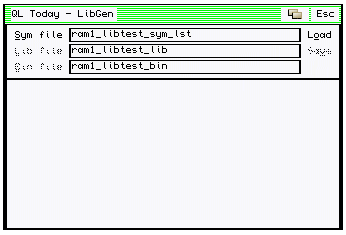
\includegraphics[width=0.65\textwidth]{Content/images/libgen_2.png}
\caption{LibGen in Action}
\label{fig:LibGenInAction}
\end{figure}


\section{The Utilities File}

In a few places in the above code, I am making calls to various
    subroutines to copy strings around, add extensions to filenames, writing
    to and getting input from various information windows etc. The following
    code is the `soon to be' library that facilitates those
    subroutines.

The first subroutine is IW\_INPUT which allows
    an information window to be used to accept input from the user.

It works by calling the WMAN\program{WMAN} routine that sets the channel ID to the
    information window in question, then copies the current value of the
    string to be edited to a working buffer. A jump back into WMAN\program{WMAN} is made to
    allow the user to edit the string. The edit may be terminated by Enter,
    ESC, Up arrow or Down arrow.

The QPTR\program{QPTR} documentation states that D0 will be zero if Enter was
    pressed, negative for any errors, and positive in ESC, Up or Down were
    used to terminate the edit. This is not true as there is no code in WMAN\program{WMAN}
    that does this. D0 will always be zero at the end of an edit, unless any
    errors occurred.

This routine attempts to follow the documentation and does set D0 to
    a positive value -{} it happens to be 1 -{} if the edit ended with a non-{}Enter
    character used to terminate it.

\begin{lstlisting}[firstnumber=1,caption={QlToday\_pe\_utilities\_asm}]
;=====================================================================
; This file contains useful utilities for a Pointer Environment
; application. It's just crying out to become a library! ;-)
;---------------------------------------------------------------------
; IW_INPUT  - Get input from a designated information window.
; IW_PRINT  - Print a string to a designated information window.
; CP_STRING - Copy a string between two locations.
; AP_STRING - Append one string to the end of another.
;=====================================================================


;=====================================================================
; IW_INPUT : accept input from an information window. The routine has
;            a working buffer of 1024 characters maximum which is
;            more than enough for any information window width.
;=====================================================================
; Entry Registers:
;
; D1.W Information window number.
; D2.L Ink colour, or negative ink colour. See WM_SWINF documentation.
; A2.L WMAN vector.
; A3.L Pointer to string.
; A4.L Pointer to work def.
;---------------------------------------------------------------------
; Exit Registers:
;
; D1.W Terminating character: Enter, Esc, Up arrow, Down arrow.
; D2.L Preserved.
; A1.L Buffer pointer.
; A2.L Preserved.
; A3.L Buffer pointer.
; A4.L Preserved.
;---------------------------------------------------------------------
; Errors:
;
; D0 = negative: Any I/O error. Old string unaffected.
; D0 = zero:     Enter terminated the edit. Old string updated.
; D0 = Positive: Another key terminated the edit. Old string updated
;                unless ESC pressed to terminate the edit.
;=====================================================================
iw_input movem.l a2-a3,-(a7)     ; Save WMAN vector & source buffer

iw_copy  lea iw_buffer,a2        ; Copy destination buffer
         bsr cp_string           ; Copy to work buffer
         move.l (a7),a2          ; Get WMAN vector

         jsr wm_swinf(a2)        ; Set channel to info window
         bne.s iw_exit           ; Bale out on error

         lea iw_buffer,a1        ; Edit buffer required in A1
         jsr wm_ename(a2)        ; Edit string in info window
         blt.s iw_exit           ; Negative is an error

;---------------------------------------------------------------------
; Bug alert. It seems at present, that this vector always returns with
; D0 set to zero or negative, but never positive. Sigh. The following
; code tries to reset that situation to how it should be, according to
; the docs.
;---------------------------------------------------------------------

         cmpi.w #27,d1           ; ESC pressed = abort edit
         beq.s iw_esc            ; Yes, all done

         move.l a3,a2            ; Original buffer is destination now
         lea iw_buffer,a3        ; New string found here
         bsr cp_string           ; Copy new value to old buffer

         cmpi.w #$0a,d1          ; Was ENTER pressed to end the edit?
         bne.s iw_esc            ; No, set D0 positive
         clr.l d0                ; Zero = ENTER was pressed
         bra.s iw_exit           ; Done

iw_esc   moveq #1,d0             ; Set D0 positive as required

iw_exit  movem.l (a7)+,a2-a3     ; Tidy WMAN vector off stack
         tst.l d0                ; Because ESC sets Z flag
         rts

;---------------------------------------------------------------------
; Working buffer for IW_INPUT.
;---------------------------------------------------------------------
iw_buffer ds.w 512+1
\end{lstlisting}

The following code prints a string to an information window. The
    information window is cleared first before printing. All the hard work is
    done by WMAN\program{WMAN}.

\begin{lstlisting}[firstnumber=last,caption={QlToday\_pe\_utilities\_asm}]
;=====================================================================
; IW_PRINT : Print a string to a designated information window.
;=====================================================================
; Entry Registers:
;
; D1.W Information window number.
; D2.L Ink colour or negative ink colour. See WM.SWINF documentation.
; A2.L WMAN vector.
; A3.L Pointer to string to be printed.
; A4.L Pointer to window working definition.
;---------------------------------------------------------------------
; Exit Registers:
;
; All registers are preserved except D0.
;---------------------------------------------------------------------
; Errors:
;
; Any I/O error.
;=====================================================================
iw_print movem.l d1-d3/a0-a1/a3,-(a7) ; Save working regsiters
         jsr wm_swinf(a2)        ; Set channel to info window
         bne.s iwp_exit          ; Bale out on error

iwp_cls  moveq #$20,d0           ; CLS
         moveq #-1,d3            ; Timeout
         trap #3                 ; Do it

iwp_prnt moveq #io_sstrg,d0      ; Send a string of bytes
         move.w (a3)+,d2         ; Byte count
         beq.s iwp_exit          ; Nothing to do
         moveq #-1,d3            ; Timeout
         exg a3,a1               ; Pointer in A1 is needed
         trap #3

iwp_exit movem.l (a7)+,d1-d3/a0-a1/a3 Restore working registers
         tst.l d0
         rts
\end{lstlisting}

The subroutine below copies a string from a location pointed to by
    A3 to the location pointed to by A2. The two locations must be holding a
    QDOS formatted string with the word count at the beginning and the bytes
    immediately following.

The code below copies byte by byte so it best suited to fairly small
    strings.

\begin{lstlisting}[firstnumber=last,caption={QlToday\_pe\_utilities\_asm}]
;=====================================================================
; CP_STRING : Copy a string from a buffer at A3.L to a buffer at A2.L.
;             The word length is always copied, even if zero.
;=====================================================================
; Entry Registers:
;
; A2.L Destination buffer address.
; A3.L Source buffer address.
;---------------------------------------------------------------------
; Exit Registers:
:
; All registers, except D0, are preserved.
;---------------------------------------------------------------------
; Errors:
;
; None. D0 is zero on exit.
;=====================================================================
cp_string
         movem.l a2-a3,-(a7)     ; Save the workers
         move.w (a3)+,d0         ; Get the source length
         move.w d0,(a2)+         ; Copy to output buffer
         beq.s cs_exit           ; Nothing more to do

         bra.s cs_next

cs_loop  move.b (a3)+,(a2)+      ; Copy one byte
cs_next  dbf d0,cs_loop          ; And all the rest

cs_exit  movem.l (a7)+,a2-a3     ; Restore the workers
         clr.l d0                ; No errors
         rts
\end{lstlisting}

And finally, for now at least, the last routine in my library (to
    be!) appends the string at A3 to the end of the string at A2. It is the
    responsibility of the programmer to ensure that enough space exists at the
    end of the destination string to hold the string being appended. The
    routine cannot check for this and assumes all will be well.

If your buffer is too small, there is a good chance that whatever
    follows the buffer will be corrupted. You have been warned!

\begin{lstlisting}[firstnumber=last,caption={QlToday\_pe\_utilities\_asm}]
;=====================================================================
; AP_STRING : Append one string to another. The destination buffer is
;             assumed to be big enough for both strings. This code
;             cannot check for this.
;=====================================================================
; Entry Registers:
;
; A2.L Destination string address.
; A3.L String to be added to A2.
;---------------------------------------------------------------------
; Exit Resisters:
;
; All regsiters, except D0, are preserved.
;---------------------------------------------------------------------
; Errors:
;
; None. D0 is zero on exit
;---------------------------------------------------------------------
ap_string
         movem.l d1/a2-a3,-(a7)  ; Save working registers
         move.w (a3)+,d0         ; Get second string size
         beq.s as_exit           ; Nothing to do, bale out

         move.w (a2),d1          ; Current length of destination
         add.w d0,(a2)+          ; Store the new length
         adda.w d1,a2            ; End of destination string
         bra.s as_next

as_loop  move.b (a3)+,(a2)+      ; Append one byte
as_next  dbf d0,as_loop          ; And all the rest

as_exit  movem.l (a7)+,d1/a2-a3  ; Restore working registers
         clr.l d0                ; No errors
         rts
\end{lstlisting}

\section{Possible Enhancements}

The program is complete and working fine as it is, however, there
    are a few enhancements that you might like to add. These could be:
\begin{itemize}[itemsep=0pt]

\item{}Add the ability to put the program to sleep. The code to do this
        is about as simple as it can be and was documented in a past article
        entitled \emph{Easy PEasy Part 2}. Failing this, you can
        examine George's EX0 example from the Easy
        PEasy\program{EasyPEasy} download.


\item{}Improve the error trapping when processing the symbol filename.
        Make sure that the correct extension is present before removing it,
        etc.


\item{}Add a loose item to close the symbol file. When closed the
        screen would be reset to its startup state and the menu removed from
        the application sub-{}window. If you do decide to attempt this, it could
        be worth waiting for the next part as you have nothing to close. But
        you could get it to clear everything out to default for now.


\item{}And anything else you may wish to add yourself.

\end{itemize}

\section{Coming Up...}
\label{ch31-the-end}%\hyperlabel{ch31-the-end}%

So, that's the end of the first part of creating a potentially
    useful utility running under the Pointer Environment. The next chapter 
    will continue from where we left off and add the rest of the
    processing.
